\section{Feature 1: Advanced OCR Implementation}

\begin{frame}{OCR: Technical Architecture}
    \begin{itemize}
        \item \textbf{Client-side Optimization}: Canvas-based image compression to ensure efficient transmission of product labels.
        \item \textbf{Image Processing}: Extraction of structured nutritional data from raw images using high-performance vision models.
        \item \textbf{Schema-driven Extraction}: Implemented JSON-schema enforcement to ensure 100\% reliability in data mapping (Calories, Sugars, Sodium, etc.).
        \item \textbf{Robust Parsing}: Developed a multi-strategy JSON recovery system to handle edge cases in model outputs.
    \end{itemize}
\end{frame}

\begin{frame}{OCR in Action}
    \begin{columns}
        \begin{column}{0.5\textwidth}
            \centering
            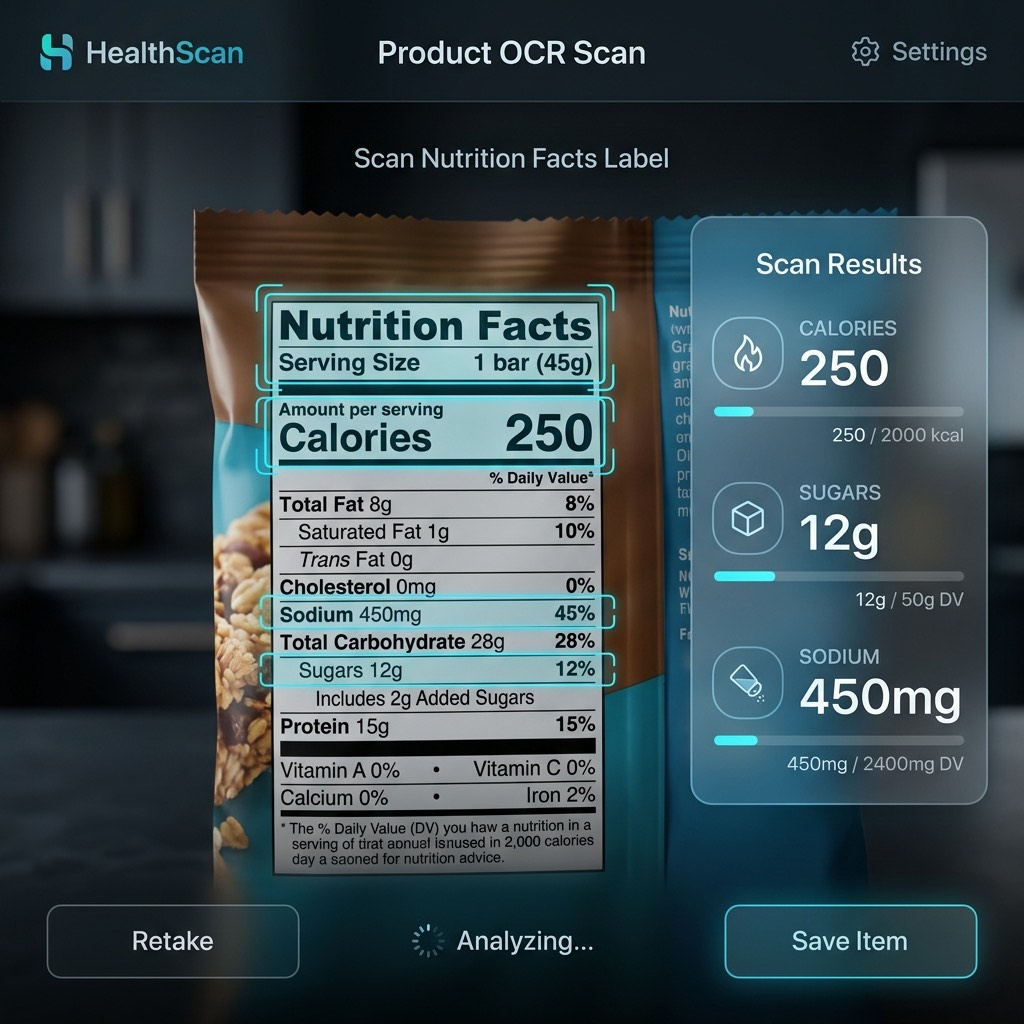
\includegraphics[width=0.8\textwidth]{healthscan_ocr_scan_1777546393550.jpg}
            \captionof{figure}{Nutrition Label OCR Scan}
        \end{column}
        \begin{column}{0.5\textwidth}
            \begin{lstlisting}[language=json, caption=Extracted Schema]
{
  "parsed_name": "Granola Bar",
  "parsed_ingredients": ["Sugar", "Oats"],
  "parsed_nutrition": {
    "calories": 250,
    "total_fat": 8,
    "sugars": 12,
    "sodium": 450
  }
}
            \end{lstlisting}
        \end{column}
    \end{columns}
\end{frame}
